\documentclass[14pt, a4paper]{extarticle}

\usepackage{geometry}
\usepackage{fancyhdr}
\usepackage{url}
\usepackage{hyperref}
\usepackage{graphicx}

\graphicspath{ {images/} }

\pagestyle{fancy}
\fancyhf{}
\rhead{\LaTeX}
\lhead{Report Healthcare Solution}
\cfoot{\thepage}

\title{Report Healthcare Solution}
\date{6-4-2017}
\author{Ruben Sol}

\begin{document}
	\nocite{*}
	\pagenumbering{gobble}
	\maketitle
	
	\newpage
	\tableofcontents
	
	\newpage
	\pagenumbering{arabic}
	\section{Introduction}
	\subsection{General Problem}
	
	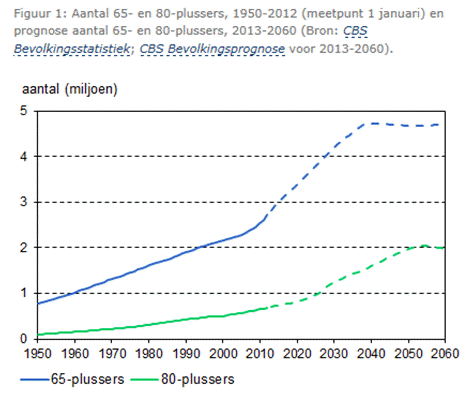
\includegraphics[scale=0.75]{vergrijzing1}
	
	
	
	The amount of elderly people is increasing quickly in the Netherlands. \cite{bevolkingspiramide} The nursing homes can't keep up with the pace and have structural issues. They don't have enough experienced staff and there are a lot of problems with the medication delivery. The elderly also feel that they don't have enough freedom. \cite{structureleproblemen}	 
	
	Because of that, there is a lot of pressure on the caregivers. If we don't reach a solution soon, there will be few places left for new elderly in nursing homes or the quality of care will be lower.
	
	\subsection{Door Problems}
	Many of the elderly have difficulities with moving through the nursing home. There are a lot of doors where for example, elderly in wheelchairs, can get stuck because the doors close to quickly. There are also doors which won't open automatically, so they require a caregiver to open it. All these problems take valuable time from the caregiver, who could be doing a lot more important things than opening doors. They also take a lot of time and trouble from the elderly. 
	
	\subsection{Emergency Alert Problems}
	There are also elderly people who have trouble with the emergency alert buttons in the nursing homes. Some of the elderly are paralyzed and have a lot of pain when they're laying in a bad position in bed at night. At those times, they can't reach the emergency alert button and have to wait till morning before they're assisted.
	
	\subsection{title}
	
	\newpage
	\section{Solution}
	
	\newpage
	\section{Concluding}
	
	\newpage
	
	\bibliography{rapport}
	\bibliographystyle{ieeetr}
	


\end{document}